% *********************************************************************
% © 2010–2022 Jeremy Sylvestre
%
% Permission is granted to copy, distribute and/or modify this document
% under the terms of the GNU Free Documentation License, Version 1.3 or
% any later version published by the Free Software Foundation; with no
% Invariant Sections, no Front-Cover Texts, and no Back-Cover Texts. A
% copy of the license is included in the appendix entitled “GNU Free
% Documentation License” that appears in the output document of this
% PreTeXt source code. All trademarks™ are the registered® marks of
% their respective owners.
%
% *********************************************************************

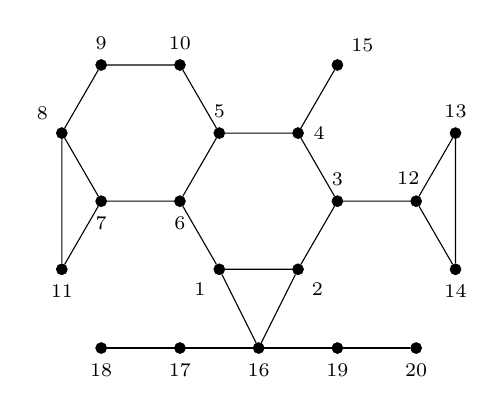
\begin{tikzpicture}[
	scale=0.5,
	vertex/.style={ circle, draw, very thin, fill, inner sep=0pt, minimum size=4pt },
	vertexg/.style={ black!40!white, circle, draw, very thin, fill, inner sep=0pt, minimum size=4pt },
	vertexo/.style={ circle, draw, very thin, inner sep=0pt, minimum size=4pt }
]

\node at (1,0) (v1) [vertex,label=below left:$\scriptstyle 1$] {};
\node at (3,0) (v2) [vertex,label=below right:$\scriptstyle 2$] {};
\node at (4,1.73) (v3) [vertex,label=above:$\scriptstyle 3$] {};
\node at (3,3.46) (v4) [vertex,label=right:$\scriptstyle 4$] {};
\node at (1,3.46) (v5) [vertex,label=above:$\scriptstyle 5$] {};
\node at (0,1.73) (v6) [vertex,label=below:$\scriptstyle 6$] {};
\draw (v1) to (v2) to (v3) to (v4) to (v5) to (v6) to (v1);

\node at (-2,1.73) (v7) [vertex,label=below:$\scriptstyle 7$] {};
\node at (-3,3.46) (v8) [vertex,label=above left:$\scriptstyle 8$] {};
\node at (-2,5.19) (v9) [vertex,label=above:$\scriptstyle 9$] {};
\node at (0,5.19) (v10) [vertex,label=above:$\scriptstyle 10$] {};
\draw (v6) to (v7) to (v8) to (v9) to (v10) to (v5);

\node at (-3,0) (v11) [vertex,label=below:$\scriptstyle 11$] {};
\draw (v8) to (v11) to (v7);

\node at (6,1.73) (v12) [vertex,label={[xshift=-0.1cm,yshift=0.01cm]$\scriptstyle 12$}] {};
\node at (7,3.46) (v13) [vertex,label=above:$\scriptstyle 13$] {};
\node at (7,0) (v14) [vertex,label=below:$\scriptstyle 14$] {};
\draw (v3) to (v12) to (v13) to (v14) to (v12);

\node at (4,5.19) (v15) [vertex,label=above right:$\scriptstyle 15$] {};
\draw (v15) to (v4);

\node at (2,-2) (v16) [vertex,label=below:$\scriptstyle 16$] {};
\node at (0,-2) (v17) [vertex,label=below:$\scriptstyle 17$] {};
\node at (-2,-2) (v18) [vertex,label=below:$\scriptstyle 18$] {};
\node at (4,-2) (v19) [vertex,label=below:$\scriptstyle 19$] {};
\node at (6,-2) (v20) [vertex,label=below:$\scriptstyle 20$] {};
\draw (v20) to (v19) to (v18) to (v17) to (v16);
\draw (v1) to (v16) to (v2);

\end{tikzpicture}
